\chapter{Quantum kinetic theory model of a continuous atom laser}
\label{KineticTheory}
\graphicspath{{Figures/KineticTheory/}{Figures/Common/}}

Continuous pumping of an atom laser is a key tool for producing superior atomic sources. Besides the obvious benefit of higher flux, it also promises improved modal stability and linewidth, much as it does for the optical laser.

The pumping process of an atom laser --- just like that of an optical laser --- is a necessarily irreversible process. This irreversibility enters through the coupling of the lasing mode to a much larger system (the reservoir). For the optical laser this reservoir is comprised of the (almost) empty modes of the de-excited atomic field of the atoms driving the lasing process. In the case of the atom laser, there are two possible choices for the reservoir providing the irreversibility: empty modes of an atomic field, or empty modes of an optical field. The former case was considered in the last chapter; the latter is the subject of this chapter\footnote{FIXME: This intro needs rewriting, but it is impossible to do so without both \chapterref{OpticalPumping} having been written and the appropriate part of the Literature Review / Background Theory chapters.}. The results presented in this chapter have been submitted for publication\footnote{FIXME: Do this.}. The results and analysis presented in \sectionref{KineticTheory:Results} of this chapter was my own work. The model presented in \sectionref{KineticTheory:Model} is based on prior work \citep{Davis:2000vn,Bijlsma:2000}. The derivation of the three-body loss term in \sectionref{MethodsAppendix:QKT3BodyLoss} and the code the results in this chapter are based on are the work of \emph{Matthew Davis}.

\section{Motivation}

Continuous pumping of an atom laser is a key tool for producing superior atomic sources. Besides the obvious benefit of higher flux, it also promises improved modal stability and linewidth, much as it does for the optical laser.

There are two essential steps towards the continuous pumping of an atom laser. The first is a delivery system for filling an atomic reservoir with ultracold atoms. The second is a process that causes at least some of those atoms to make an irreversible, atom-stimulated transition into the BEC.

Continuous delivery of ultracold atoms has been demonstrated in a number of experiments\footnote{FIXME: Add citations.}, and is an important component of thermal atomic interferometry experiments. FIXME: Complete paragraph.

The atom-stimulated transitions into the condensate can be made irreversible by coupling to a reservoir. There are two possible reservoirs: the empty modes of the electromagnetic field accessible via a transition from an excited atomic state, or the empty modes of the atomic field accessible via evaporation. Having considered the former in \chapterref{OpticalPumping} it is the latter under consideration in this chapter.

Sequential reloading of a target BEC was achieved using optical tweezers \citep{Chikkatur:2002qa}, where a series of source condensates were added adiabatically by manipulating the trapping potentials, and excitations were subsequently removed by continuous evaporation. This milestone experiment maintained the condensate fraction, and therefore the potential flux of a potential atom laser. An atom laser produced from such an experiment would, however, not possess the desired narrow linewidth as the source condensates used were of a similar size to or larger than the condensate being replenished causing significant scattering into modes other than the target condensate. To produce an atom laser with a narrow linewidth it would be necessary for the atomic source to negligibly disrupt the target condensate. While this could be achieved by merging the target condensate with significantly smaller condensates more frequently, it is technically very challenging to develop high flux sources of Bose-condensed atoms compared to sources at higher temperature, which have a higher average flux. In this chapter it is shown that a similar experiment using an ultra-cold \emph{thermal} source ought to be able to pump the target BEC and maintain a significant BEC population using a phase-preserving Bose-enhanced process.

%This method has the advantage that it can be performed without the presence of resonant light, but the obvious disadvantage that it relies on the system approaching thermal equilibrium, and will therefore be reversed by the addition of atoms above the condensate temperature. In this chapter it is demonstrated that a driven system undergoing evaporative cooling can produce a high-flux, phase-stable atom laser for a range of experimental parameters.

\section{Scheme}
\label{KineticTheory:Scheme}

\begin{figure}
    \centering
        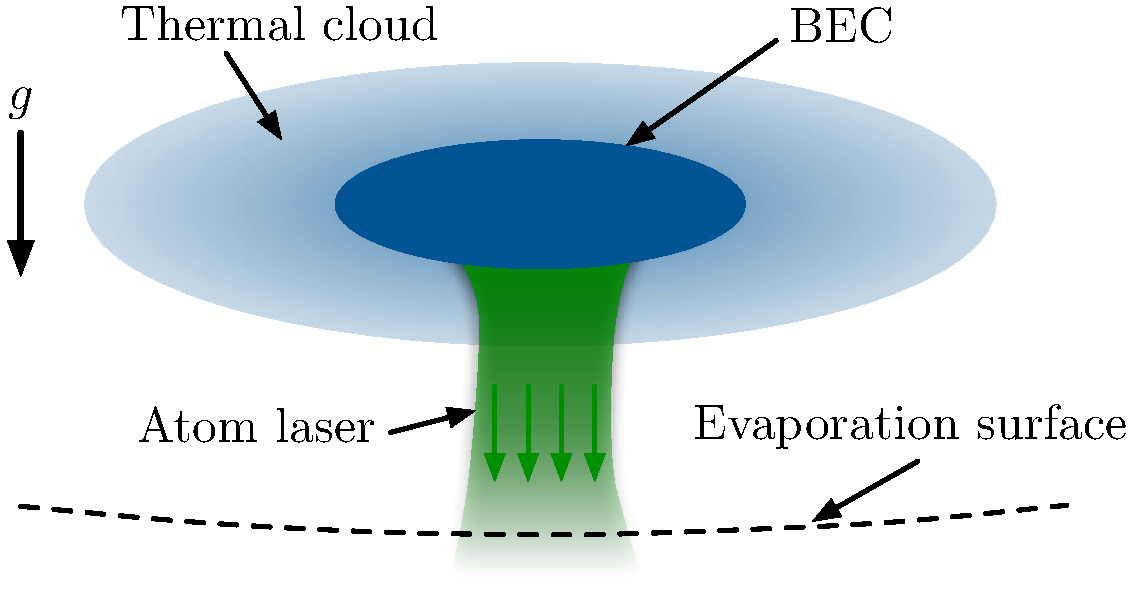
\includegraphics[width=10cm]{QKTScheme}
    \caption{Schematic of the experimental setup.}
    \label{KineticTheory:QKTScheme}
\end{figure}

The proposed scheme for a pumped atom laser is illustrated in \figureref{KineticTheory:QKTScheme} and is very similar to the processes used to evaporate a thermal cloud to condensation in a magnetic trap and produce a (quasi-continuous) atom laser. The additional element in this scheme is a process for replenishing the cloud of thermal atoms in the trap.  

In this scheme the gain process for the condensate is the same Bose-enhanced scattering between thermal atoms and the condensate that drives condensate growth when evaporating to produce condensate \citep{Gardiner:1997kx,Davis:2000vn,Bijlsma:2000}.  This process becomes irreversible when one of the scattered atoms has enough energy to cross the evaporation surface and be removed from the thermal cloud.  The loss of atoms from the thermal cloud is balanced by a replenishment process that couples the thermal cloud to a source of atoms at finite temperature.

The atom laser beam itself is to be produced by large momentum-transfer Raman outcoupling from the condensate to minimise the loss from the atom laser as it traverses the evaporation surface\footnote{An alternative configuration would be to place the evaporation surface \emph{above} the thermal cloud, however the effectiveness of the evaporation surface is reduced as its contact area with the thermal cloud is reduced. In a typical trap with a trapping frequency of $\omega = 2\pi \times \unit[100]{Hz}$ in the vertical direction and an aspect ratio of $10$, the separation between the centre of the condensate and the centre of the magnetic trap and the evaporation surface is $y_\text{sag} = \unit[25]{\micro m}$.  For a thermal cloud of $N=10^6$ rubidium atoms at the critical temperature, the $1/e$ radius in the vertical direction is $y_\text{thermal} = \unit[17.3]{\micro m}$. Placing the evaporation surface above the thermal cloud would then significantly reduce its contact area with the thermal cloud. For this reason the evaporation surface in \figureref{KineticTheory:QKTScheme} has been pictured below the thermal cloud.}. To minimise direct outcoupling from the thermal cloud, the two Raman lasers used in the outcoupling process can be focussed to only intersect in the immediate vicinity of the condensate.

A dynamic equilibrium will be reached when the rate of atom loss from the condensate due to outcoupling balances the rate of atoms gained due to scattering with the thermal cloud.  If the evaporative surface is tuned so that atoms of energy $\varepsilon_\text{cut}$ and higher are rapidly and continually removed from the trap, then all collisions that give atoms energy greater than $\varepsilon_\text{cut}$ will become irreversible. As $\varepsilon_\text{cut}$ is lowered, a larger fraction of the scattering processes that leave atoms in the condensate mode will become irreversible. This suggests that there must be some value of $\varepsilon_\text{cut}$ for which the condensate experiences net gain. What is not clear is whether the net gain can proceed efficiently, i.e. on a timescale much shorter than other losses from the condensate.  Lowering $\varepsilon_\text{cut}$ also reduces the total number of thermal atoms present. In the limit that $\varepsilon_\text{cut}$ reaches the condensate energy, there will be no background gas at all, and the condensate cannot experience net gain.  We therefore expect that for a given set of parameters, there will be an optimal value for $\varepsilon_\text{cut}$ that maximises the net gain, which may or may not be positive. In order to examine this issue, quantum kinetic theory (QKT) \citep{Gardiner:1997tz,Jaksch:1997ug,Gardiner:1998wx,Jaksch:1998sj,Gardiner:2000ug,Lee:2000vs,Davis:2000vn} has been employed, which has been effective in describing the growth of condensates \citep{Davis:2000vn}.

\section{Model}
\label{KineticTheory:Model}

\begin{figure}
    \centering
        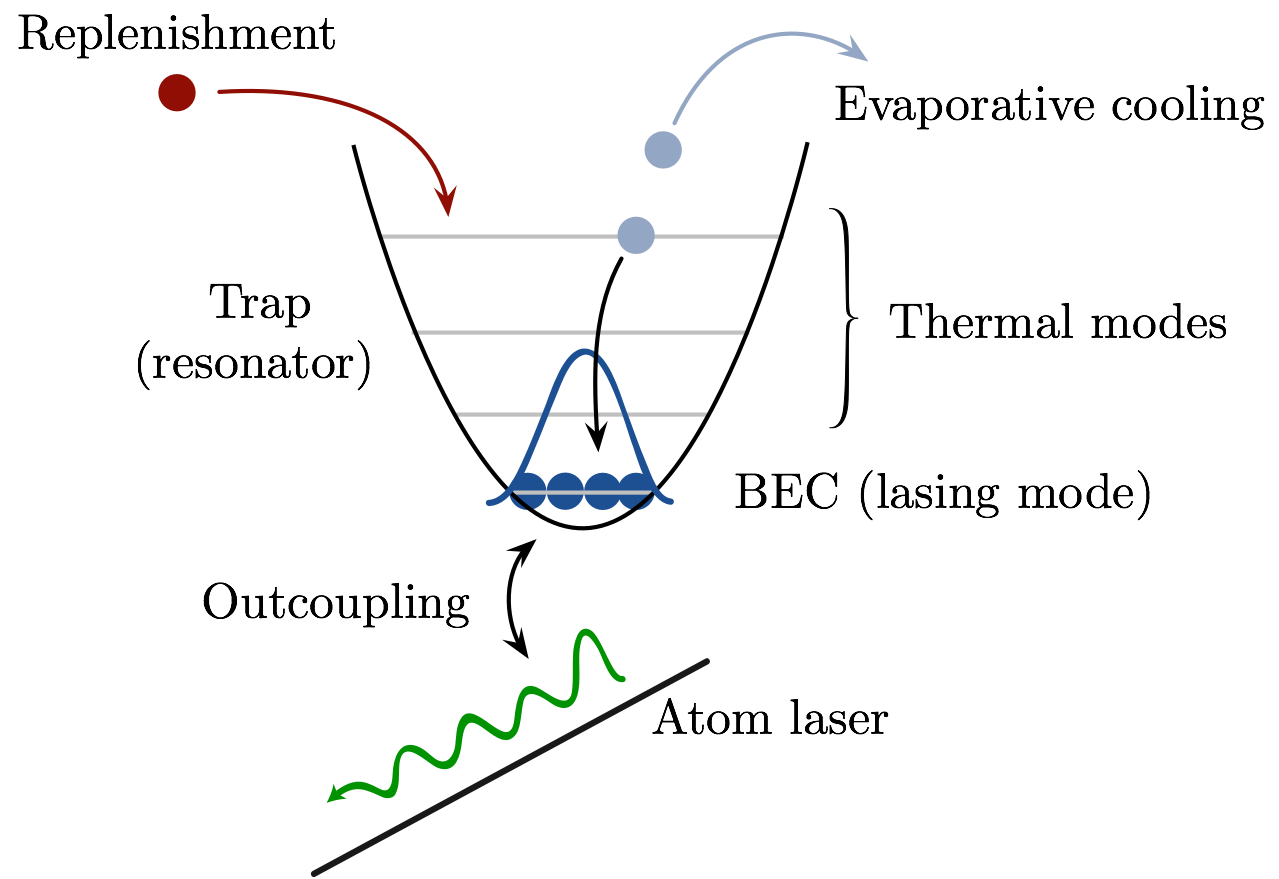
\includegraphics[width=10cm]{QKTModel2}
    \caption{Schematic of the theoretical model.}
    \label{KineticTheory:QKTModel}
\end{figure}

The theoretical model described in this section is an extension of the kinetic model of \citet{Bijlsma:2000}, which was successfully used to study condensate growth in an experiment in which a cloud of thermal atoms just above condensation temperature were shock-cooled below transition \citep{Miesner:1998}.  After the shock-cooling the atoms were left to equilibrate, the condensate formation being driven by the same collisional processes that would drive condensate growth in the proposed pumped atom laser experiment described in the previous section.  To fully describe this proposed experiment, the kinetic model of \citeauthor{Bijlsma:2000} must be modified to include the effects of the replenishment and outcoupling processes illustrated in \figureref{KineticTheory:QKTScheme}. 

Another important process that must be included in the model is three-body recombination (the dominant loss process in typical BEC experiments \citep{Burt:1997fk}). In the absence of this process, there would be no need to evaporate to form a condensate. As the condensation temperature $T_C$ is proportional to $N^{\frac{1}{3}}$, the condensate \emph{fraction} increases as the total number of trapped atoms increases. In fact, once a condensate forms the thermal cloud would cease to grow and each atom added to the trap would increase the equilibrium condensate number by one\footnote{As the condensation temperature is proportional to $N^{\frac{1}{3}}$, and the condensate fraction in a harmonic trap is $\displaystyle \frac{N_0}{N} = 1 - \left(\frac{T}{T_C}\right)^3$ for $T < T_C$, the number of atoms in the condensate is given by $N_0 = N - \alpha T^3$ for some constant $\alpha$ depending on the trap geometry (negative condensate numbers correspond to $T > T_C$).}. The reason that this is not a feasible method of achieving condensation is that the number of atoms at room temperature required to form a condensate in a typical magnetic trap is $N \sim 10^{30}$. The density at the centre of such a trap that the timescale for particle loss due to three-body loss would be of the order of (FIXME: insert timescale)! Any realistic model of a pumped atom laser must therefore include the effect of three-body recombination.

\parasep

The starting point of kinetic model presented here is to treat separately the thermal and condensed components of the system in \figureref{KineticTheory:QKTScheme}. The condensate is assumed to be adiabatically-evolving and well-described by a Thomas-Fermi distribution. The condensate dynamics are then fully described by the number condensed atoms $N_0(t)$. The thermal cloud is assumed to be well described within the Hartree-Fock approximation as comprised of single particles in the effective potential of the harmonic trap plus condensate mean field. This thermal cloud is then described by its energy distribution function $g(\varepsilon, t)$ and the density of states $\rho(\varepsilon, t)$. The time-dependence of the density of states comes from the inclusion of the effect of the mean field of the condensate on the thermal atoms. The density of states is then fully determined by the trap geometry and the condensate number $N_0(t)$.

The equations of motion for the model can be written in the following form, separating the contributions of the processes involved,
\begin{align}
    \frac{d N_0}{d t} =\begin{split}
        &\relphantom{+}\left. \frac{d N_0}{d t}\right|_\text{thermal--condensate} \\
        &+\left. \frac{d N_0}{d t}\right|_\text{3-body loss} \\
        &+\left. \frac{d N_0}{d t}\right|_\text{outcoupling}
    \end{split},
    & \frac{\partial (\rho g)}{\partial t} = \begin{split}
        &\relphantom{+}\left. \frac{\partial (\rho g)}{\partial t}\right|_\text{thermal--thermal} \\
        &+\left. \frac{\partial (\rho g)}{\partial t}\right|_\text{thermal--condensate} \\
        &+\left. \frac{\partial (\rho g)}{\partial t}\right|_\text{3-body loss} \\
        &+\left. \frac{\partial (\rho g)}{\partial t}\right|_\text{replenishment} \\
        &+\left. \frac{\partial (\rho g)}{\partial t}\right|_\text{redistribution}
    \end{split},
    \label{KineticTheory:EvolutionEquations}
\end{align}
where the subscripts `thermal--thermal' and `thermal--condensate' denote collisional processes between atoms in the corresponding states (\figureref{KineticTheory:ProcessDiagrams}(a) and (b), respectively), the subscript `3-body loss' indicates the contribution due to three-body recombination processes, the subscript `replenishment' indicates the contribution due to the replenishment of the thermal cloud (\figureref{KineticTheory:ProcessDiagrams}(d)), the subscript `outcoupling' indicates the contribution due to outcoupling from the condensate to form the atom laser (\figureref{KineticTheory:ProcessDiagrams}(e)), and the subscript `redistribution' indicates the contribution due to the redistribution of energy levels due to changes in the mean-field of the condensate (\figureref{KineticTheory:ProcessDiagrams}(c)). It is assumed that atoms with energy greater than the evaporative energy cut-off $\varepsilon_\text{cut}$ are removed from the system sufficiently quickly that it can be assumed that $g(\varepsilon > \varepsilon_\text{cut}) = 0$.

\begin{figure}
    \centering
    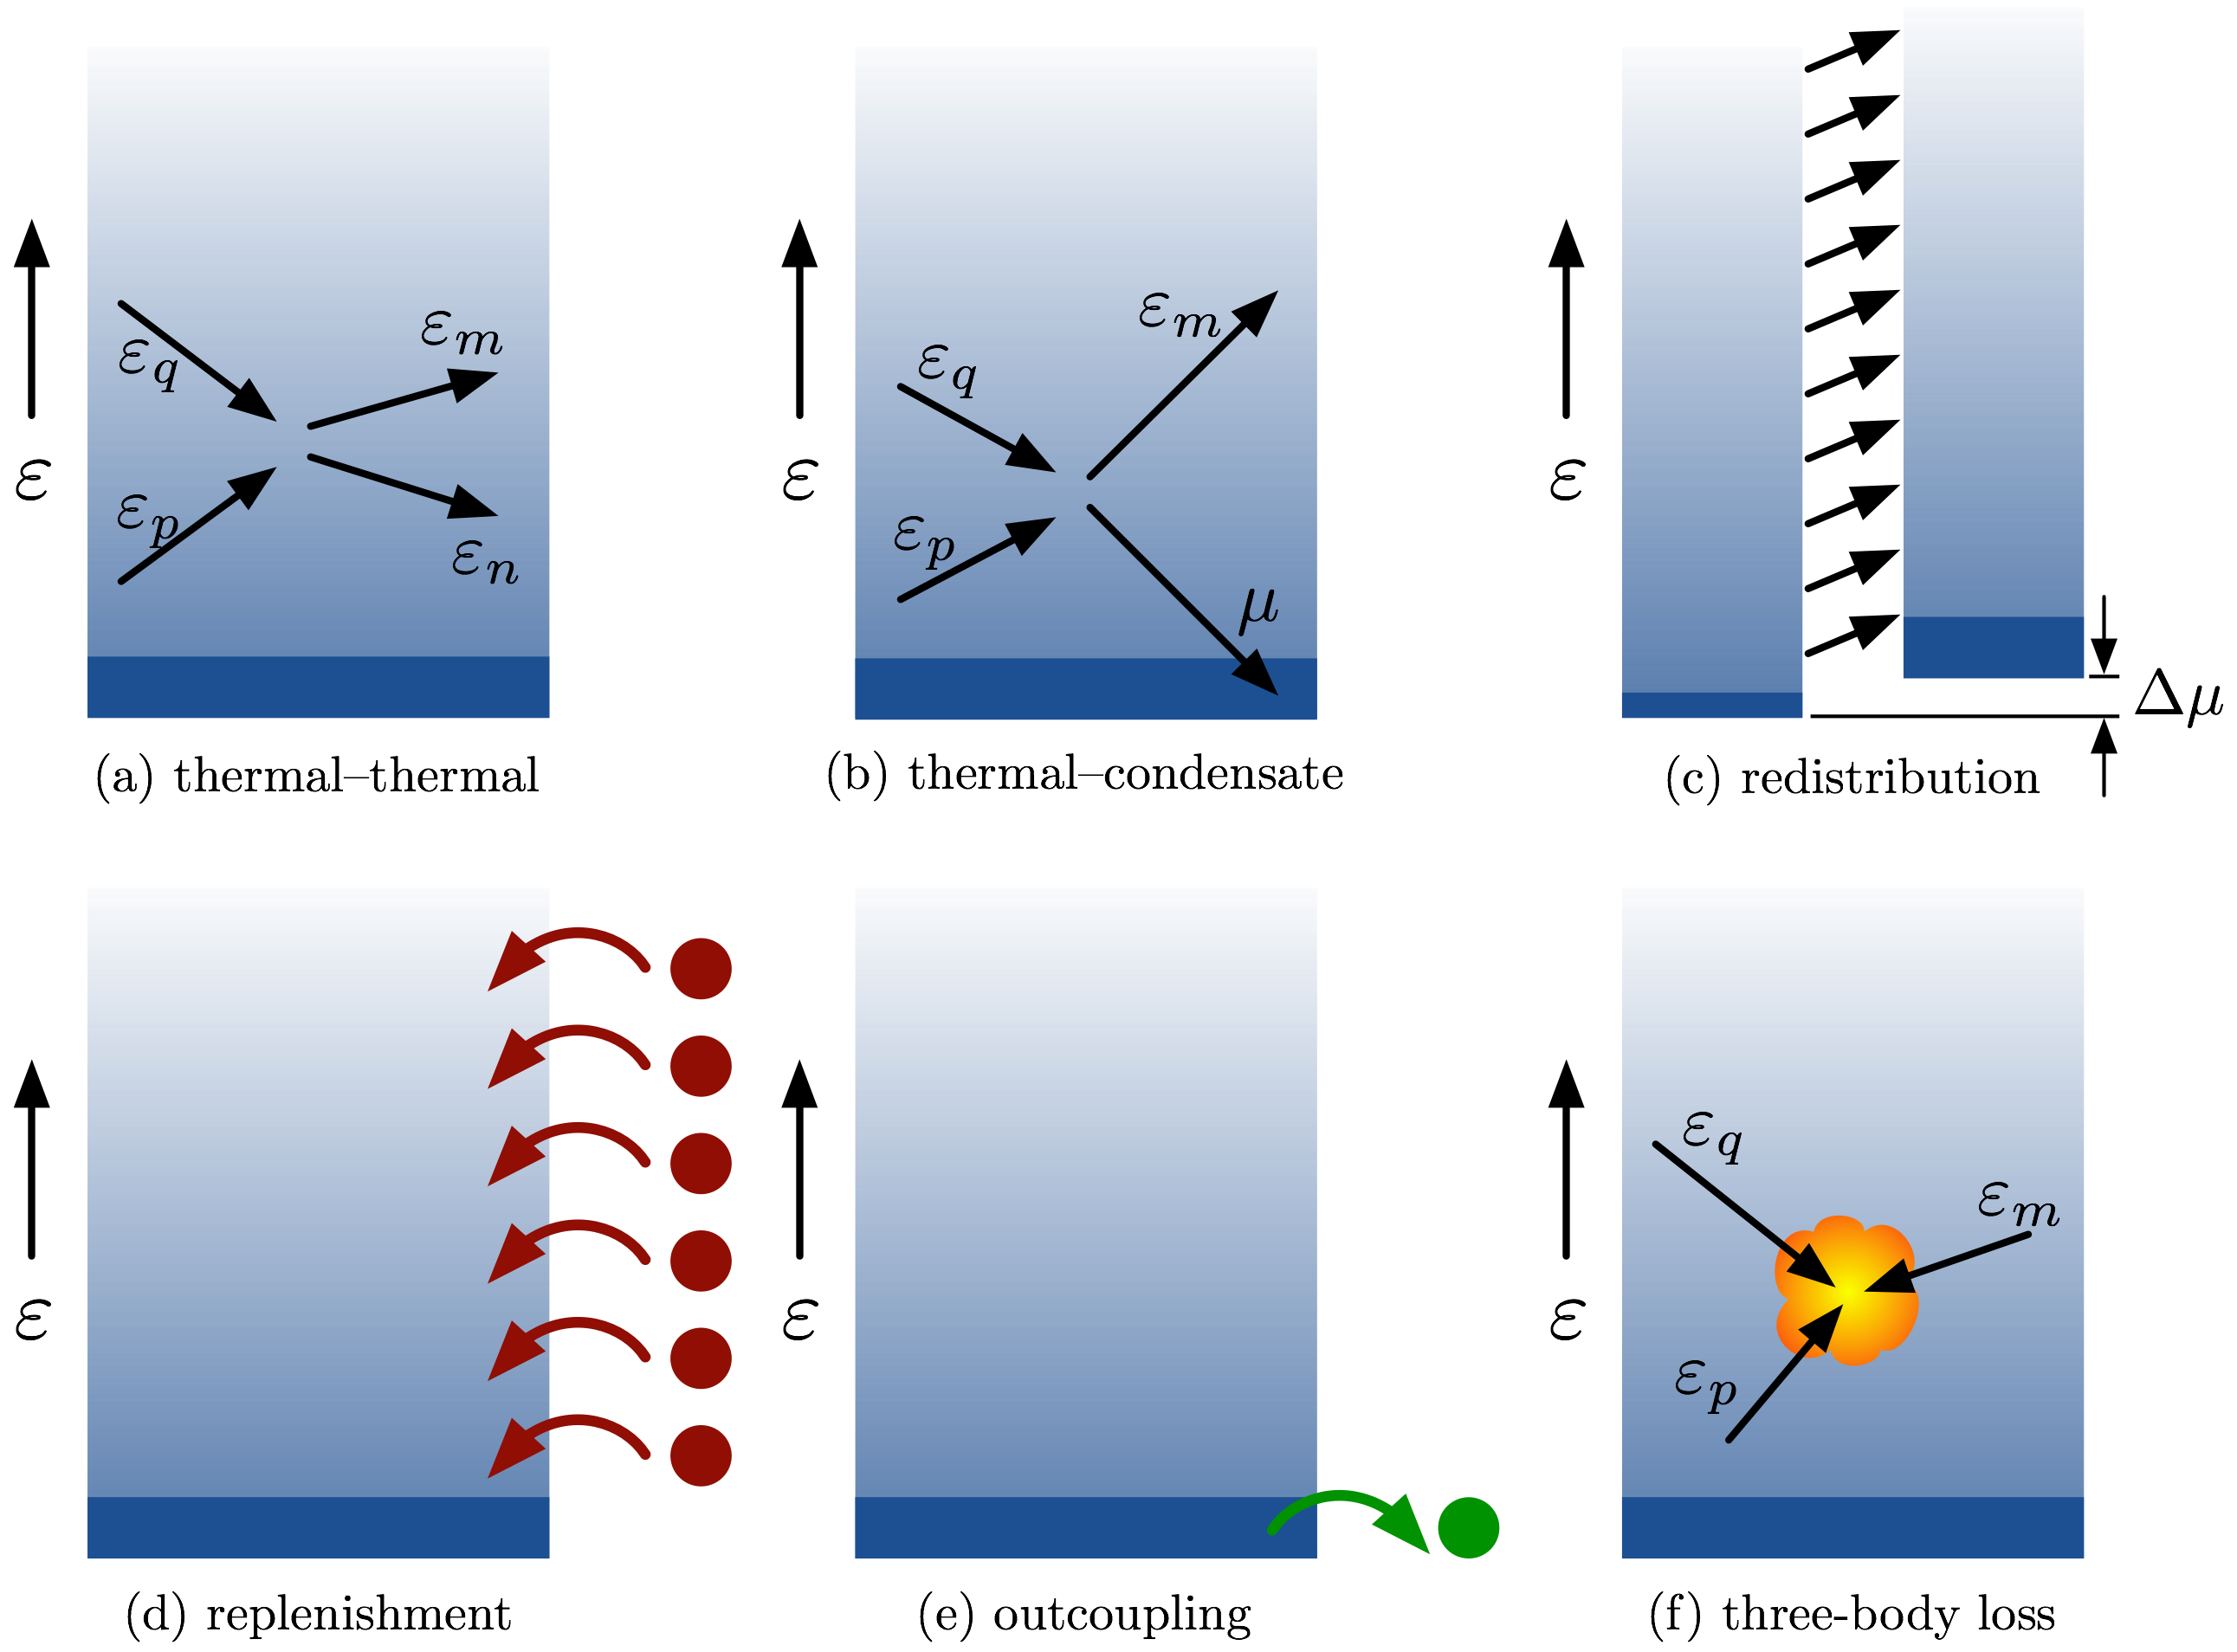
\includegraphics[width=14cm]{ProcessDiagrams}
    \caption{Schematic of the primary processes involved in the evolution of the model described in \eqref{KineticTheory:EvolutionEquations}. The bottom rectangle represents the condensate at $\varepsilon = \mu(t)$. FIXME: Caption.}
    \label{KineticTheory:ProcessDiagrams}
\end{figure}

Derivations of the `thermal--thermal', `thermal--condensate' and `redistribution' terms in \eqref{KineticTheory:EvolutionEquations} are given in \citep{Bijlsma:2000}. The outcoupling process from the condensate is modelled as a simple linear loss process with corresponding rate constant $\gamma$,
\begin{align}
    \left.\frac{d N_0}{d t}\right|_\text{outcoupling} &= - \gamma N_0.
    \label{KineticTheory:OutcouplingProcess}
\end{align}
The thermal cloud is modelled as being continuously replenished from a source that provides a constant flux $\Phi$ of atoms at a temperature $T$. For simplicity it is assumed that each energy level $\varepsilon$ in the source is coupled directly to the level in the thermal cloud with energy $\varepsilon + \mu(t)$\footnote{FIXME: $\mu(t)$ has not been defined.}, i.e. the lowest energy level of the source ($\varepsilon=0$) is coupled directly to the lowest energy level in the trap ($\varepsilon = \mu(t)$). This simple model gives the form of the contribution due to replenishment as
\begin{align}
    \left. \frac{\partial \big(\rho(\varepsilon, t) g(\varepsilon, t))}{\partial t} \right|_\text{replenishment} &= \Gamma \rho_0(\varepsilon - \mu(t)) g_T(\varepsilon - \mu(t)),
    \label{KineticTheory:ReplenishmentProcess}
\end{align}
where $\rho_0(\varepsilon)$ is the density of states in the absence of a condensate, $g_T(\varepsilon)$ is the Bose-Einstein energy distribution at temperature $T$, and $\Gamma$ is a rate constant such that
\begin{align}
    \Gamma \int_0^\infty \rho_0(\varepsilon) g_T(\varepsilon)\, d\varepsilon = \Phi,
    \label{KineticTheory:GammaPhiRelation}
\end{align}
where the integral is defined over all energies as $\Phi$ is defined to be the \emph{total} flux of atoms from the source before evaporation. The derivation of the contributions to \eqref{KineticTheory:EvolutionEquations} due to three body loss were performed by \emph{Matthew Davis}, and are covered in \sectionref{MethodsAppendix:QKT3BodyLoss}.
%While this is perhaps an unreasonable assumption, it means that we can easily determine the steady state of the system.

FIXME: Write and clean up this paragraph. In obtaining this model a number of assumptions are made:
\begin{enumerate}[(i)]
    \item Ergodic
    \item Adiabatic evolution of the condensate. This also applies at the evaporation cutoff.
    \item Neglect of the anomalous density.
    \item Neglect of the thermal density in the effect on the condensate profile and the density of states.
    \item Energy scales are such that all non-condensate excitations are particle-like not phonon-like (use of Hartree-Fock mean-field).
    \item Evaporation occurs on a time-scale faster than collisions.
\end{enumerate}
These approximations are discussed at length in a comprehensive review article \citep{Proukakis:2008} in which the QKT formalism is referred to as the `ZNG' theory.

The computer code used to solve \eqref{KineticTheory:EvolutionEquations} was written by \emph{Matthew Davis}.

\section{Results}
\label{KineticTheory:Results}
This is my contribution. Example simulations demonstrating time-dependence of the distributions, the dependence on $\eta$. Behaviour (and simple model in high-temperature limit) in the presence of three-body loss.

Joe has suggested that we not rely on the high-temperature limit, but I would really, really like to have that in.

We need a plan for the story that goes in this chapter. This story, and the accompanying graphs are what will be needed to construct the poster for FINESS.

Somewhere we list the full parameters of the model, $T$, $\Phi$, $\gamma$ and $\varepsilon_\text{cut} = \eta k_B T$.

\subsection{Typical results and parameter studies}
Here we illustrate the time-dependence of a typical solution, and consider the dependence on each parameter. The dependence on most are trivial; only $\eta$ is non-trivial. Awaiting supercomputer results.



\subsection{Behaviour in the high-temperature limit}
Although it would be possible to create a pumped atom laser by combining condensates in a manner similar to the experiment by \citet{Chikkatur:2002qa}, such an atom laser would have significantly reduced phase-stability unless the replenishment process were essentially continuous. However, to replenish a condensate by collisional interactions with a continuous source of condensed atoms, the replenishment source would itself need to have many of the desired properties of a pumped atom laser! Instead, it would be preferable to use a source \emph{above} condensation temperature for replenishment.

We consider now the experimentally-relevant limit of replenishing the thermal cloud using a high-flux thermal source of atoms. For such sources, two simplifications are possible. First, for temperatures greater than $T_C$ the Bose-Einstein energy distribution of the source $g_T(\varepsilon)$ is well approximated by the Boltzmann distribution $g_T(\varepsilon) \approx \zeta e^{-\beta \varepsilon}$ for some constant $\zeta$, and $\beta = \left(k_B T\right)^{-1}$. Secondly, for high temperature sources the optimum evaporation cut-off $\varepsilon_\text{cut}$ will be much smaller than the characteristic energy of the source $k_B T$, and hence $\displaystyle \eta = \frac{\varepsilon_\text{cut}}{k_B T} \ll 1$.  From these simplifications it can be seen that the energy distribution below the evaporation cut-off is well described by the single parameter $\zeta$ as $g_T(\varepsilon \leq \varepsilon_\text{cut}) \approx \zeta$.

At this point, no overall simplification has occurred as we have simply rewritten the temperature dependence of the atomic source in terms of the parameter $\zeta$. However, as the energy distribution of the atomic source only appears in \eqref{KineticTheory:ReplenishmentProcess}, its only influence on the system dynamics will be through the combined quantity $\kappa = \Gamma \zeta$. An expression for $\kappa$ directly in terms of relevant experimental quantities can be obtained by using the definition \eqref{KineticTheory:GammaPhiRelation},
\begin{align}
    \Phi &= \Gamma \int_0^\infty \rho_0(\varepsilon) g_T(\varepsilon)\, d\varepsilon\\
    &= \Gamma \int_0^\infty \frac{\varepsilon^2}{2 (\hbar \overline{\omega})^3} \zeta e^{-\beta \varepsilon}\, d\varepsilon\\
    &= \Gamma \zeta \frac{1}{2 (\hbar \overline{\omega})^3} \int_0^\infty \varepsilon^2 e^{-\beta \varepsilon}\, d\varepsilon\\
    &= \left(\frac{k_B T}{\hbar \overline{\omega}}\right)^3 \Gamma \zeta\\
    \kappa &= \Gamma \zeta = \Phi \left(\frac{\hbar \overline{\omega}}{k_B T}\right)^3
\end{align}
where $\overline{\omega} = \left(\omega_x \omega_y \omega_z\right)^{\frac{1}{3}}$ is the geometric mean of the trapping frequencies, and $\displaystyle\rho_0(\varepsilon) = \frac{\varepsilon^2}{2 (\hbar \overline{\omega})^3}$ is the density of states in a harmonic trap in the absence of a condensate \citep{PethickSmith}.

The quantity $\kappa$ is a figure-of-merit for the thermal source. It quantifies the qualitative behaviour already known: for the same atomic flux $\Phi$, a source with a lower temperature will result in a larger condensate (FIXME: see some figure); and for the same temperature, a source with a higher atomic flux will also result in a larger condensate (FIXME: see some other figure). Our interest is in determining what values of $\kappa$ are necessary to produce a pumped atom laser, and whether such values are achievable.

For the limit of high-temperature atomic sources, we have reduced the four variables $(\Phi, T, \varepsilon_\text{cut}, \gamma)$ required to define the model \eqref{KineticTheory:EvolutionEquations} down to three $(\kappa, \varepsilon_\text{cut}, \gamma)$. Of these three, our main interest is in the dependence of the system on the properties of the atomic source through $\kappa$. In contrast, the dependence of the equilibrium condensate number on the outcoupling rate $\gamma$ is well understood and the results would not be expected to change qualitatively with $\gamma$. It is therefore appropriate to choose a representative value for the outcoupling rate (here $\gamma = \unit[0.3]{s\textsuperscript{-1}}$) and focus on the remaining two quantities.

As discussed in the previous section, there is an optimal choice for the evaporation cut-off $\varepsilon_\text{cut}$. Our interest here is in the best-case scenario: for a given thermal source, what is the largest condensate we can produce? To examine this question and to verify that $\kappa$ does fully describe the properties of the thermal source in the appropriate limit we have performed a parameter scan of the model \eqref{KineticTheory:EvolutionEquations} for a range of fluxes $\Phi$ and temperatures $T$ of the atomic source, for each combination determining the optimum evaporative cut $\varepsilon_\text{cut}$ to give the largest steady-state condensate number. The results of this parameter study are displayed in \figureref{KineticTheory:FigureOfMerit}.

\begin{figure}
    \centering
    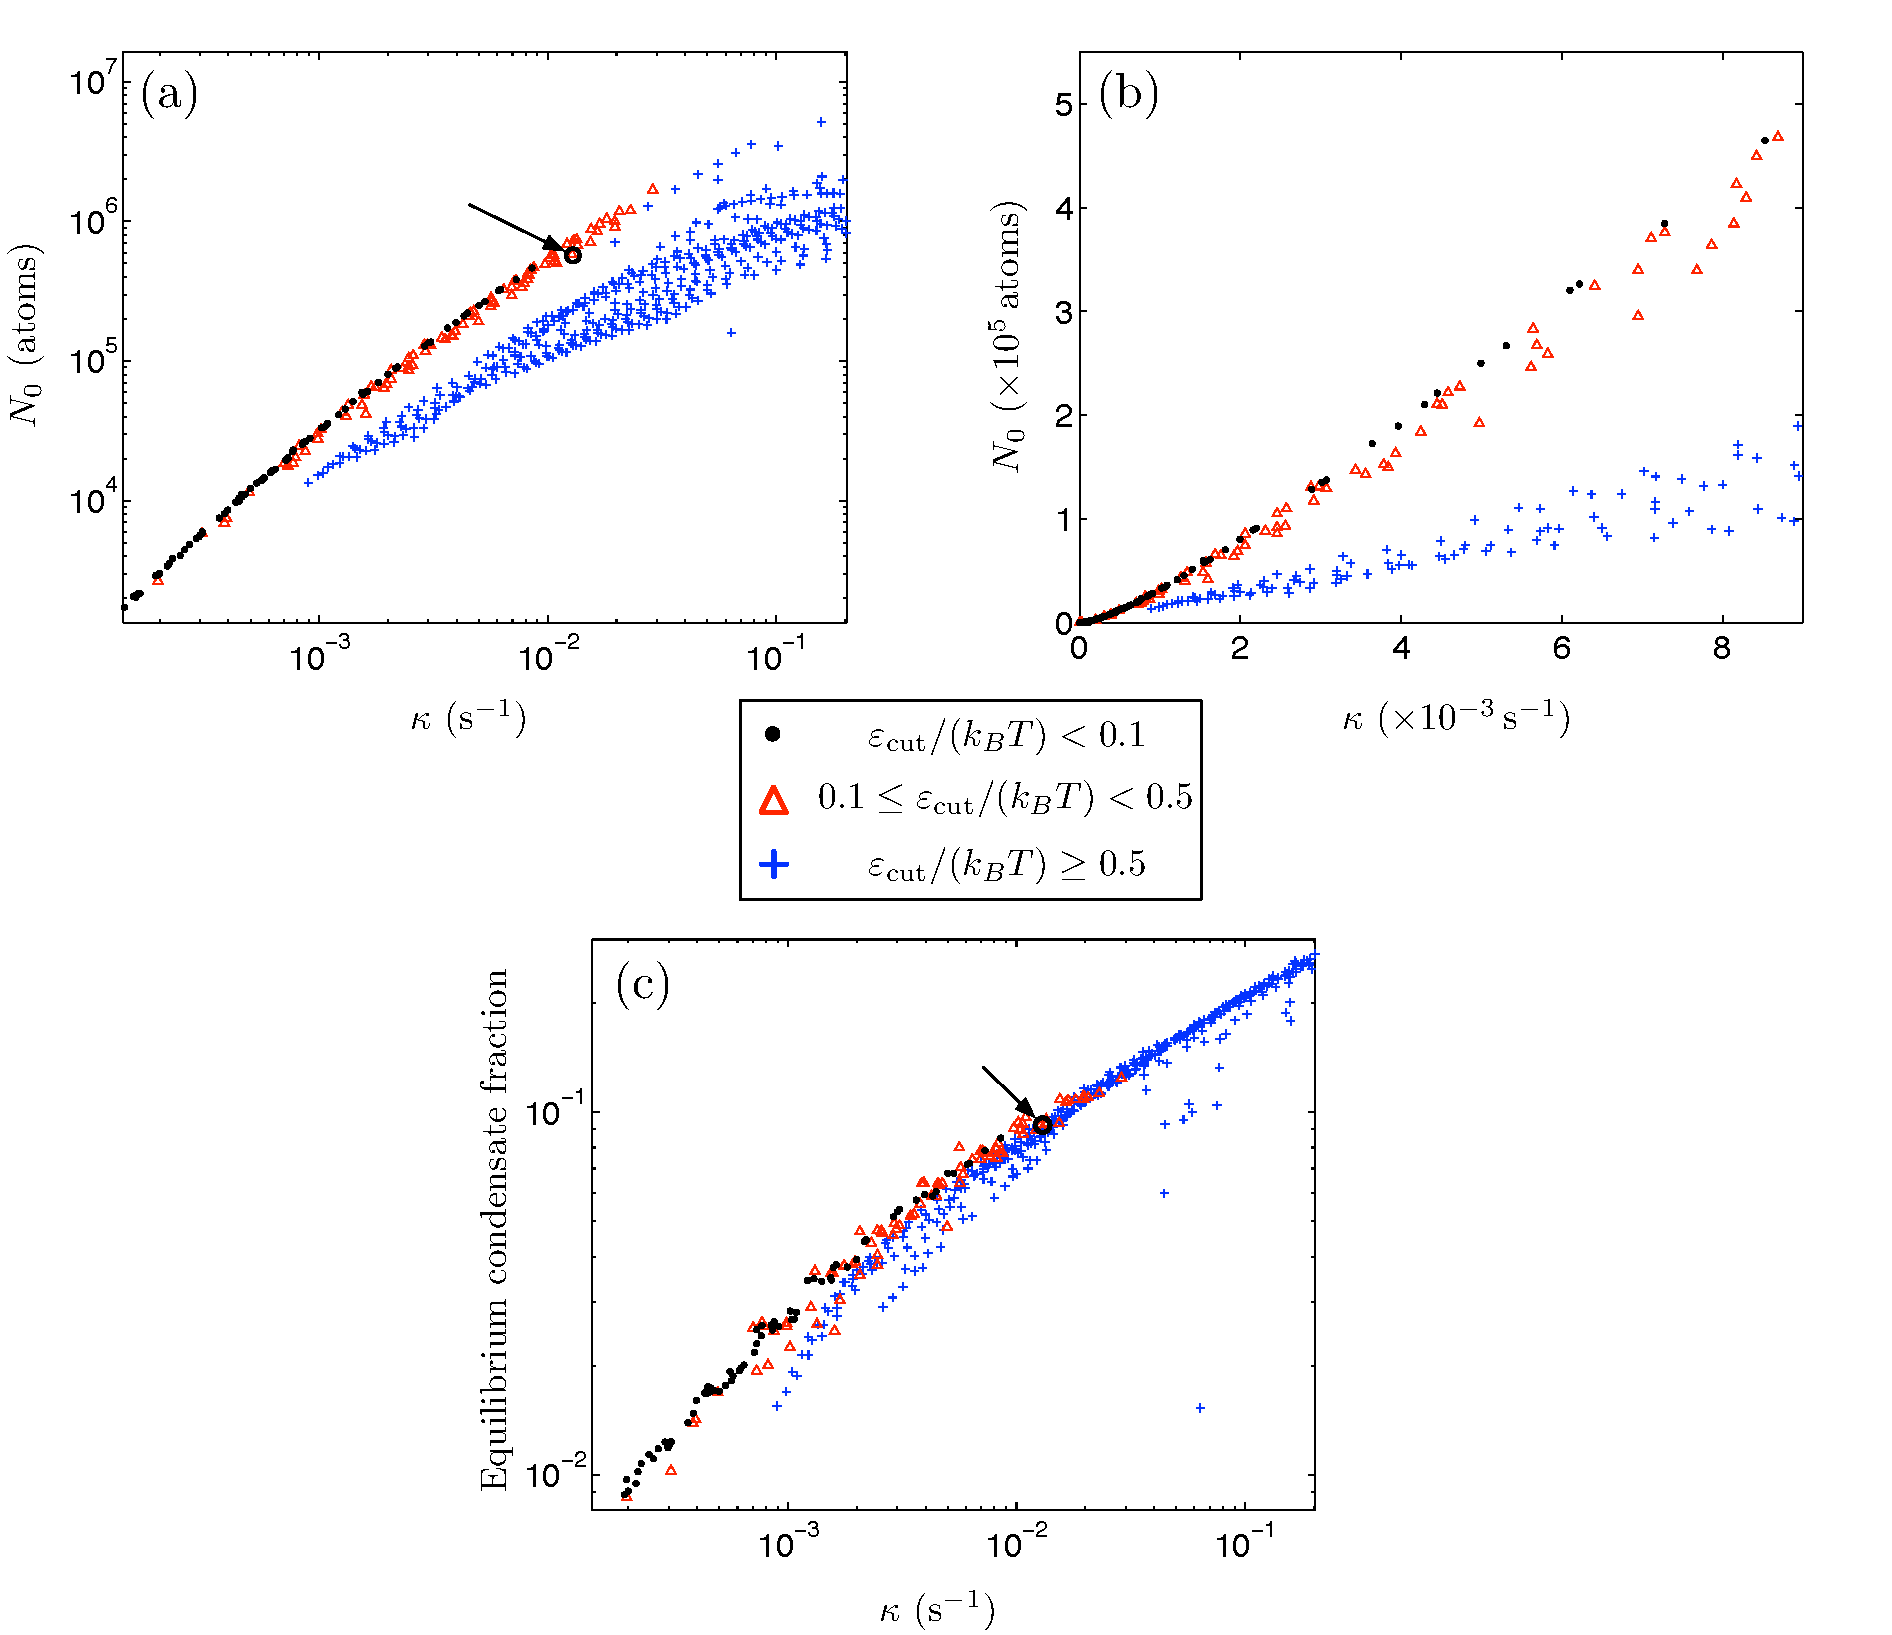
\includegraphics[width=15cm]{FigureOfMerit}
    \caption{FIXME: Figure caption. Plot of equilibrium $N_0$ against $\kappa$ for $\eta < 0.1$ (black), $0.1 < \eta < 0.5$ (red) and $\eta > 0.5$ (blue). Or something like that.}
    \label{KineticTheory:FigureOfMerit}
\end{figure}

\begin{figure}
    \centering
    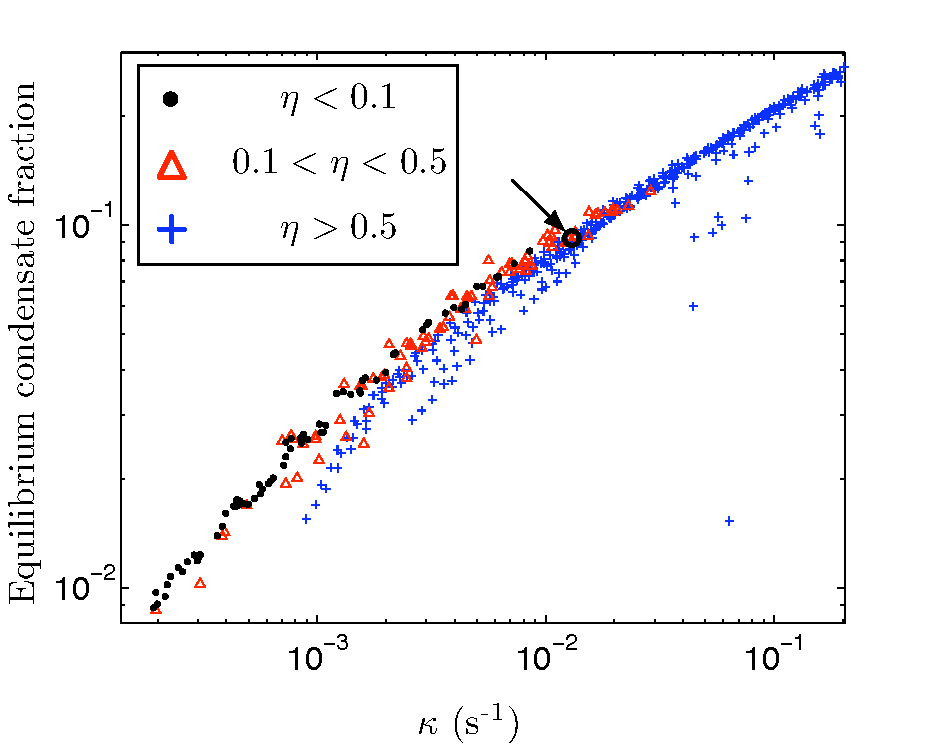
\includegraphics[width=7cm]{CondensateFraction}
    \caption{FIXME: Figure caption. Plot of equilibrium condensate fraction against $\kappa$ for the usual suspects.}
    \label{KineticTheory:CondensateFraction}
\end{figure}

and to verify that $\kappa$ does fully describe the properties of the thermal source in the appropriate limit we have performed a parameter scan over the space $(\Phi, T, \varepsilon_\text{cut})$, choosing $\gamma = \unit[0.3]{s\textsuperscript{-1}}$ as noted above.



There are a number of high-flux atomic sources that have been developed both for the production of BEC and, more recently, in the consideration of atom-interferometry using cold thermal atomic beams. Such `cold' atomic sources range from Zeeman slowers, MOT's, LVIS configurations, etc. The aim of this chapter is to examine the feasibility of the use of such thermal atomic sources in the production of high-flux continuous, degenerate atomic sources. Studying this limit

Creating

The most experimentally interesting case

The most experimentally rele


Talk about various high-flux atomic sources that could be used. If it weren't for three-body loss, it wouldn't much matter and we could just do whatever. But. 


The limit that is of the greatest experimental relevance is that of replenishing a condensate with high-flux sources well above condensation temperature.

high-flux sources


To facilitate extracting useful information from this model, we consider the experimentally relevant limit of high-flux replenishment sources far above condensation temperature. Although a complete analytic model cannot be obtained in this limit, we can recognise an equivalence between difference sources. For such high-temperature sources, the Bose-Einstein distribution is well approximated by the Boltzmann distribution $g_B(\varepsilon) = A e^{-\beta\varepsilon}$ for some constant $A$, and $\beta = \left(k_B T\right)^{-1}$. For such high-temperature sources, the optimum choice of the evaporation cut-off $\varepsilon_\text{cut}$ will be small compared to stuff. This will mean that $\eta$ will be small. If $g_B(\varepsilon_\text{cut}) = A e^{-\eta} \approx g_B(0)$, then the thermal source is completely described by the parameter $K=\Phi A$.




In the limit of a reservoir of high-temperature atoms, we can make some useful statements and comparisons.


In the limit of high-temperature 


This is the main contribution of the paper. We study the behaviour in the high temperature limit, obtain a simple model, verify the model and then compare against experiment.




\section{Conclusion}
Thermal sources must be close to degenerate to be useful. 